\documentclass[a4paper,14pt]{extarticle}
\usepackage{cmap}				% To be able to copy-paste russian text from pdf			
\usepackage[utf8]{inputenc}
\usepackage[T1]{fontenc}
\usepackage[margin=1in]{geometry}
\usepackage[english]{babel}

\usepackage[hyphens]{url}
\urlstyle{same}
\usepackage{hyperref}

\usepackage{multirow}
\usepackage{graphicx}
\usepackage{caption}
\usepackage{eurosym}

\usepackage{libertine}
\usepackage{libertinust1math}

\usepackage[style=alphabetic, backend=biber]{biblatex}
\addbibresource{fx.bib}
\renewcommand*{\bibfont}{\small}
\setcounter{biburllcpenalty}{9000}
\setcounter{biburlucpenalty}{9500}

\author{Artem Bakulin}
\date{Translation: \today. Original: September 16, 2019}

\title{Foreign Exchange Market}

\begin{document}

\maketitle
\thispagestyle{empty}

\begin{figure}[h]
\centering
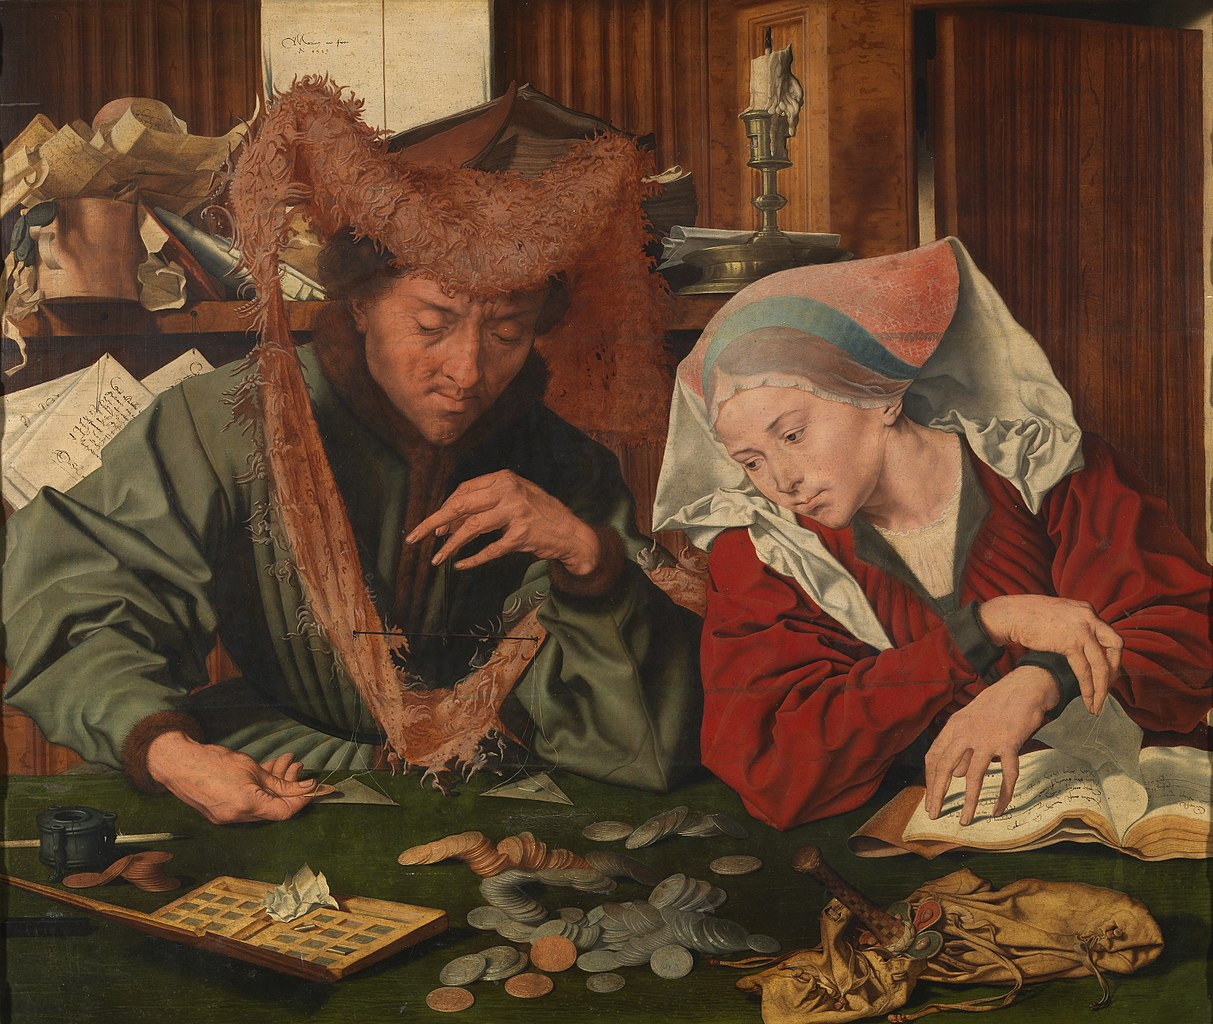
\includegraphics[width=\textwidth]{../moneychanger_and_his_wife.jpg}
\captionsetup{labelformat=empty}
\caption{\footnotesize{
Marinus van Reymerswaele. \href{https://commons.wikimedia.org/wiki/File:Marinus_Claesz._van_Reymerswaele_001.jpg}{The moneychanger and his wife (1539)}. Museo del Prado, Madrid.
}}
\end{figure}
\newpage

\section*{Introduction}

I joined  Deutsche Bank as a Java programmer in 2009 (the
Great Recession, the Miracle on the Hudson, ``Slumdog Millionaire'', the swine 
flu outbreak, the Russian national football team's defeat in the World Cup 
qualification). During the interview, I was informed that I would be working on 
the AutobahnFX project.

FX? Foreign Exchange? My knowledge of the currency market was no different from 
that of an average layman. There is a currency exchange kiosk at the corner near 
my house, but the difference between buying and selling rates always gives me
a nervous tic. There is advertisement of Forex dealers in every subway car. 
Newspapers depict investment banks as either all-knowing speculators who 
predict currency rates for years ahead, or a bunch of incompetent money-grubbers 
who crashed the global economy. ``Well, okay,'' I thought, ``I'll have to figure 
it out.''

This article is part of what I discovered while working on various systems. Why 
should you read it? Firstly, it is interesting. The modern currency market is a 
complex distributed system with numerous independent actors. Secondly, if you 
work in finance, you may find similarities with other markets, from the bond 
market to weather derivatives market. Lastly, it will be easier for you to 
read the debrief in the press when another investment bank goes bust next time.

Here is our plan. In this article, I will explain how the foreign exchange 
market works, what role major investment banks play, what services they provide 
to clients, what risks they take, and how they eventually make money. In the 
second article we will discuss whether the market can operate differently and 
what could happen if banks were prohibited from engaging in this business. You 
can proceed directly to the second article in case you are familiar with terms 
market-maker, limit order book, market risk and over-the-counter market.

\section*{Clients and Market Makers}

Let's start our discussion of the currency market with a German company 
``Berlinische Motoren Wagen AG''. They have recently sold a batch of cars to
the United States, and now they wish to convert part of their dollar revenue 
into euros. There is nothing easier: all they need to do is contact their bank. 
If the treasurer of ``BMWagen'' decides to use the phone, which is not uncommon 
even in the 21st century, the following dialogue will take place between him 
and someone from the bank:

--- Guten Tag. This is ``BMWagen'' calling. Euro-dollar, 10, please.

--- Guten Tag. Our price is 56--58.

--- Bought. Vielen Dank.

What just happened? First, the client indicated that they were interested in a 
transaction worth 10 million euros in the euro-dollar currency pair. The 
transaction size is usually stated in the first currency of the pair, and the 
word ``million'' is usually implied, because respectable business-people are not 
interested in smaller amounts. Notice that the client did not specify whether 
they intended to buy or sell euros.

The bank responds with a two-way quote: they are willing to buy euros from the 
client at 56 and sell euros to the client at 58. The numbers 56 and 58 may seem 
unusual when it comes to the exchange of euros for dollars, because we all know 
that the euro-dollar exchange rate is closer to 1 than to 50. However, these 
are not the entire exchange rates but only a part of them. If the euro-dollar 
exchange rate is around 1.09 today, there is no need to mention the cumbersome 
``figures'' 1.09 in every conversation. Professionals are already aware of that. 
It is enough to mention the third and fourth digits after the decimal point, 
known as ``pips''. Therefore, the quote 56--58 indicates the bank's willingness 
to buy euros at the rate of 1.09\underline{56} and sell euros at the rate of 
1.09\underline{58}.

Finally, the client communicates their decision: they are buying 10 million 
euros from the bank at the rate of 1.0958, which means they pay 10\,958\,000 
dollars to the bank and receive 10\,000\,000 euros in return. Theoretically, the 
client could have said ``sell'' and entered into the opposite transaction: 
paying 10\,000\,000 euros and receiving 10\,956\,000 dollars. They could also 
choose to decline the transaction altogether, mutter something like ``these 
capitalists have gotten too audacious'', and hang up.

Perhaps you noticed that neither the client nor the bank mentioned the 
settlement date. Usually, the seller and the buyer agree on the exchange rate 
today, and the transfer of funds between accounts takes place on the second 
business day. This ``default'' settlement date is called the ``spot date'' or 
simply the ``spot''. Accordingly, a transaction with settlement on the spot date 
is called a spot transaction. In principle, the client can ask to settle on any 
other convenient day, but that would no longer be a spot transaction but a 
forward, which we will discuss another time.

Let's cover a bit more terminology. The rate 1.09\underline{56} at which the 
bank buys euros is called the bid rate. The rate 1.09\underline{58} at which the 
bank is selling is called the ask or offer rate. The difference between them, 
0.00\underline{02} or 2 pips, is called the spread. The arithmetic mean of the 
bid and the ask rates, 1.09\underline{57}, is called the mid or mid rate.

A financial company that provides its clients with two-way quotes on currency or 
other assets is called a ``market maker'', because it literally makes prices out 
of thin air. Two other terms that are used interchangeably with market maker in 
this context are ``dealer'' and ``liquidity provider''. A market maker doesn't 
have to be a bank, although 8 out of the top 10 market makers in the foreign 
exchange market are indeed international investment banks. The top three 
leaders, accounting for a quarter of the market, are JPMorgan, Deutsche, and 
Citi \cite{euromoney2019}.

The profit of a market maker is the difference between the bid and the ask 
rates. It is easy to calculate that if the bank sold 10 million euros to the 
client at 58 and then bought euros from another client at 56, it would earn 
$10\,000\,000 \cdot (1.09\underline{58} - 1.09\underline{56}) = 2\,000$ dollars
due to the difference in rates.

Sometimes I'm asked if a bank can sell euros which it currently doesn't have. 
Yes, with caveats and within certain limits, this is possible. As we already 
know, currency transactions are usually settled on the second business day, 
rather than immediately. Therefore, a bank can start with a zero balance, sell 
euros which it doesn't have, and then buy euros from another client.

So far, it doesn't seem too complicated, does it? We have all seen exchange rate 
boards with euro and dollar rates so many times that any random person on the 
street can easily explain at what rate you can buy dollars and at what rate you 
can sell them. If a bank operates as a large exchange office basically, 
then what's so difficult about it? Buying at a lower price, selling at a higher 
price, earning the spread --- any five-year-old can handle that. At a certain 
level of abstraction, that's true, but there is a nuance.

\section*{Managing Market Risk}

What can go wrong in a simple and elegant strategy of a market-maker? The answer 
is straightforward: unexpected market movements can leave it without any profit 
and even result in losses. The possibility of losing money due to changes in 
market prices is called market risk.

Imagine that you are a market maker. You sold 10 million euros to ``BMWagen'' at 
a rate of 1.09\underline{58}, and now you are waiting for the next client who 
would sell you euros at 56. But this second client went on a lunch break, so 
you, as traders say, are ``in a position''. Suddenly, a news flash comes in: the 
European Central Bank (ECB) is winding down its quantitative easing program. 
While you are trying to figure out what that means, the market has already 
reacted: other banks are quoting rates of 86--88, 30 pips higher than before. 
When the second client returns from lunch, they won't sell euros to you at 56. 
You will have to offer them a price of at least 86 to prevent them from going to 
your competitors. What's the bottom line? You bought 10 million at 86 and sold 
at 58. Congratulations, you have just lost \$28\,000. Please do not do that 
again.

How can a market maker protect themselves from such losses? The first and most 
obvious solution is to widen the spread between the bid and the ask. If you had 
offered ``BMWagen'' a spread of 62 pips (26--88) rather than 2 pips (56--58),
then even a 30-pips market move would have allowed you to earn \$1\,000 by 
selling at 88 and buying at 87. Unfortunately for market makers, clients don't 
like wide spreads and will gladly go to competitors if their spreads are better.

The second option is to make your price more attractive for those clients who 
are selling. If you have just sold at 58, you can quote 56.5--58.5 for the 
following client, even if the market mid-rate is still 57. This type of quote is 
called skewed. What's the point? The bid 56.5 became more favorable, and if the 
client is simultaneously talking to a couple of other market makers, they are 
more likely to sell euros to you. You will eliminate the risk and earn \$1\,500. 
It's less than the \$2\,000 of the full spread, but still not bad. On the other 
hand, the ask price of 58.5 became worse, and you essentially discourage the 
client from buying euros from you at all, so that they don't increase your risk.

Finally, the third approach is to ``close'' the position in the interbank 
market. Banks make prices not only for clients but also for each other. You can 
call another market maker, get a quote from them with a narrower spread, let's 
say 56.0--57.5, and buy the required 10 million euros at 57.5. This way, you 
will lock in a profit of \$500.

An attentive reader will notice that the quote of 56.0--57.5 was skewed to the 
left relative to the mid-rate of 57. Apparently, the second market maker 
recently bought euros from their client and is now employing strategy number 2, 
trying their best to prompt you to make a deal that will help them exit their 
position. In this way, two market makers can make a deal that allows both to 
lock in a profit.

By combining all three methods (managing the spread, incentivizing clients to 
reduce risk, closing positions in the market), a market maker can earn their 
penny with an acceptable level of risk. This penny is not guaranteed, and each 
specific transaction can result in a loss, but it is still possible to make the 
money in the long run. It's sufficient to always keep the current position in 
mind, by how much it can be increased, how much it would cost to close it in the 
market, which clients are likely to approach soon, in which direction they 
usually trade, whether it's time to provide skewed prices, what spread would be 
justified given the current market volatility, whether an ECB press conference 
is expected within 15 minutes, whether there is correlation between positions in 
euro-dollar and euro-pound pairs, and a few other similar details.

If you're wondering whether it is possible to offload at least some of this work 
to a computer, then you are thinking in the right direction.

\section*{Interbank Market}

Let's take a look at how computers help banks trade with each other when they 
need to close a position in the market. The two largest platforms that automate 
interbank trading are \href{https://www.cmegroup.com/trading/market-tech-and-data-services/ebs.html}{Electronic Brokerage Services (EBS)}
and
\href{https://www.refinitiv.com/en/products/spot-matching-forwards-matching}{Reuters Matching}.
Both platforms operate on similar principles, and their market shares are 
approximately equal \cite{golov2019fx}. Historically, certain currency pairs are 
traded more on EBS, while others are traded on Reuters. I will discuss EBS 
because the majority of euro-dollar transactions take place there.

All trades on the EBS platform go through a Central Limit Order Book 
(CLOB). Any company can 
send its limit order through an application or API. To do this, three 
parameters need to be specified: the direction of the trade (buy or sell), the 
size, and the desired exchange rate. For example, ``buy 1 million at a rate of 
1.09\underline{56}5 or lower'' or ``sell 1 million at a rate of 
1.09\underline{57}5 or higher''. Orders can also be canceled or modified at any 
time.

The EBS server collects the orders, arranges them by desired price (buy orders 
in descending order, sell orders in ascending order), and disseminates a summary 
to all trading participants, as shown in Table \ref{clob_table}.

\begin{table}[h]
\centering
\begin{tabular}{l|l|l|l|l}
\multirow{2}{*}{Level} & \multicolumn{2}{c|}{Buyers} &
\multicolumn{2}{c}{Sellers} \\ \cline{2-5}
& Price & Size & Price & Size \\ \hline
1 & 1.09\underline{56}5 & \euro1m & 1.09\underline{57}5 & \euro2m \\
2 & 1.09\underline{56}4 & \euro2m & 1.09\underline{57}6 & \euro3m \\
3 & 1.09\underline{56}3 & \euro7m & 1.09\underline{57}7 & \euro6m \\
4 & 1.09\underline{56}2 & \euro8m & 1.09\underline{57}8 & \euro7m \\
5 & 1.09\underline{56}1 & \euro9m & 1.09\underline{57}9 & \euro6m
\end{tabular}
\caption{Order book for euro-dollar currency pair}
\label{clob_table}
\end{table}

It's worth noting that the order book is anonymous. Nobody, except EBS, knows 
who is that mysterious stranger that is willing to sell 2 million 
euros at 1.09\underline{57}5. We cannot even determine whether we see a single 
order for 2 million or two orders for 1 million each from two different market 
participants.

The best bid at a price of 56.5 and the best ask at a price of 57.5 form the 
market spread (also known as the best bid/offer, BBO). Unlike a market maker's 
two-sided quote, these two prices may come from two different counterparties, 
but this is not essential. For us, it looks like if someone gave us a quote of 
56.5--57.5 with a 1 pip spread.

For example, suppose we want to sell 1 million euros. In this case we can send 
an order stating ``we sell 1 million at a rate of 1.09\underline{56}5 or 
higher.'' The system will determine that our new order can be matched with an 
existing buyer's order, and it will automatically execute the trade between us.

In order to make a deal immediately, we will have to give a discount to the 
buyer. We will be selling euros at 56.5 when the mid-rate is 57.0, i.e. 
slightly cheaper. For a trade size of 1 million, this will cost us $1\,000\,
000\cdot(1.09\underline{56}5 - 1.09\underline{57}0) = -50$ dollars. In traders' 
jargon, this is called ``crossing the spread'' or ``paying the spread''. 
Strictly speaking, we will only pay half of the full spread 56.5--57.5, but it 
is more common to say ``pay the spread'' rather than ``pay the half-spread''.

Let's return to the example of closing a position when we wanted to buy 10 
million euros. We won't be able to execute a similarly advantageous trade with a 
narrow 1 pip spread, because we can only buy 2 million at 57.5, not 10 million. 
The remaining 8 million will cost us more. We will send an order to EBS stating 
``buy 10 million at 1.09\underline{58} or lower''. Since several companies have 
already expressed their willingness to sell at this rate, EBS will start 
matching our order with them, moving from top to bottom in the order book. This 
way, we will buy 2 million at 57.5, then another 3 million at 57.6, and 5 
million at 57.7. The state of the order book after our purchase of 10 million is 
shown in Table \ref{clob_table_2}.

\begin{table}[h]
\centering
\begin{tabular}{l|l|l|l|l}
\multirow{2}{*}{Level} & \multicolumn{2}{c|}{Buyers} &
\multicolumn{2}{c}{Sellers} \\ \cline{2-5}
& Price & Size & Price & Size \\ \hline
1 & 1.09\underline{56}5 & \euro1m & 1.09\underline{57}7 & \euro1m \\
2 & 1.09\underline{56}4 & \euro2m & 1.09\underline{57}8 & \euro7m \\
3 & 1.09\underline{56}3 & \euro7m & 1.09\underline{57}9 & \euro6m \\
4 & 1.09\underline{56}2 & \euro8m & & \\
5 & 1.09\underline{56}1 & \euro9m & &
\end{tabular}
\caption{Limit order book from Table \ref{clob_table} after executing an order
``buy 10 million at 1.09\underline{58} or lower''}
\label{clob_table_2}
\end{table}

Interestingly, our trades have just moved the market. Initially, the top two 
bids and asks were at rates of 56.5--57.5, with a mid-rate of 57.0. Now, the 
first level of orders shows prices of 56.5--57.7, and the mid-rate is 57.1.

But that's not all. Immediately after the trade, EBS will send an updated order 
book and anonymized information about recent trades to all market participants 
(``three trades have just took place at rates of 1.09575, 57.6, and 57.7''). 
Other participants will quickly match the changes in the order book with the 
trades, and will deduce that someone was very eager to buy euros and didn't 
hesitate to pay the spread and eat three levels of selling orders. Does 
he know something important? Someone might decide that the fair rate has 
increased and move their orders higher. For example, a buyer with an order for 1 
million at 56.5 may adjust it slightly up by 0.2 pips to 56.7. The market spread 
will again be 1 pip (56.7--57.7), but around the increased mid-rate of 57.2. 
This is how the invisible hand of the market works: an active buyer pushes  
the market price up.

Let's calculate the cost of our purchase. The weighted average buying rate is 
calculated as $(2 \cdot 57.5 + 3 \cdot 57.6 + 5 \cdot 57.7)/10 = 57.63$ pips. 
Once again, we paid the spread to others by buying euros above the mid-rate of 
1.09\underline{57}. This amounts to $10\,000\,000 \cdot (1.09\underline{57} - 
1.09\underline{57}63) = -630$ dollars, or 63 dollars per million. On the other 
hand, we sold euros to the client at 58.0, so our profit will be $10\,000\,000 
\cdot (1.09\underline{58} - 1.09\underline{57}63) = 370$ dollars.

Is there any way to reverse the situation and make others pay the spread to us? 
No problem. To do that, we need to join the queue of buyers by entering 
an order ``buy 10 million at 1.09\underline{56}5 or lower''. This will 
create an order book as shown in Table \ref{clob_table_3}.

\begin{table}[h]
\centering
\begin{tabular}{l|l|l|l|l}
\multirow{2}{*}{Level} & \multicolumn{2}{c|}{Buyers} &
\multicolumn{2}{c}{Sellers} \\ \cline{2-5}
& Price & Size & Price & Size \\ \hline
1 & 1.09\underline{56}5 & \euro11m & 1.09\underline{57}5 & \euro2m \\
2 & 1.09\underline{56}4 & \euro2m  & 1.09\underline{57}6 & \euro3m \\
3 & 1.09\underline{56}3 & \euro7m  & 1.09\underline{57}7 & \euro6m \\
4 & 1.09\underline{56}2 & \euro8m  & 1.09\underline{57}8 & \euro7m \\
5 & 1.09\underline{56}1 & \euro9m  & 1.09\underline{57}9 & \euro6m
\end{tabular}
\caption{Limit order book from Table \ref{clob_table} after submitting an order 
``buy 10 million at 1.09\underline{56}5 or lower''.}
\label{clob_table_3}
\end{table}

We just have to wait a little for an active seller who would be willing 
to pay the spread and sell euros at 56.5. When the platform starts matching 
orders, the first million will go to the person who entered the queue with an 
order at 56.5 before us, but all the subsequent millions will be ours. If we 
manage to sell all 10 million at 56.5, we will earn $10\,000\,000 \cdot 
(1.09\underline{57}0 - 1.09\underline{56}5) = 500$ dollars, or 50 dollars per 
million.

The drawback of this passive strategy of placing an order and waiting is the 
complete uncertainty of execution time. The seller willing to transact at 56.5 
can show up in 10 milliseconds, in a minute, or never. Remember that we entered 
the market to hedge the risk of selling euros to the client at a rate of 58.0. 
If we wait too long for the buy order at 56.5 to be executed, we might end up 
waiting till the ECB press conference and a 30-pip jump. It would 
be extremely frustrating to realize that we could have eliminated the risk for 
just 630 dollars but chose to save a bit and ended up losing much more. 
Therefore, we need to weigh the cost savings on the spread against the risk of 
untimely execution of limit orders.

\section*{Counterparty Risk and Market Segmentation}

The computerized market built around the order book looks promising. All 
market participants, not just selected market-makers, can submit their orders. 
One could expect that competition among sellers will lower prices in sell 
orders, while competition among buyers will raise prices in buy orders. As a 
result, the market spread, at least for small transactions, will be narrower, 
and many companies will find it more advantageous to execute trades through EBS 
rather than relying on market-makers. Unfortunately, things are not that simple.

EBS and Reuters operate as broker-like intermediaries. When the EBS system 
matches a buyer and a seller, for example Deutsche and JPMorgan, a bilateral 
transaction occurs directly between these companies. The role of the trading 
platform owner is similar to that of a real estate agent: to help the buyer and 
the seller find each other, charge them a fee for the service, but by 
no means become a party to the agreement. In economic terms, the counterparty 
credit risk falls on the seller and the buyer.

What is counterparty credit risk? Let's say, as in the example above, we 
purchased 10 million euros on EBS at an average price of 57.63. For simplicity, 
let's assume that all 10 million euros were bought from a single seller. We 
expect to receive 10 million euros from this seller on the second working day 
and immediately transfer them to our client, ``BMWagen''. The client will pay us
\$10\,958\,000, and we will pay \$10\,957\,630 pay to the seller on EBS . Our 
euro payments will cancel out, and we will make a profit of \$370. 

If the seller from EBS goes bankrupt, we will have a problem. We still need 10 
million euros, which we will have to buy from the market at the new market rate. 
It would be fine if the market rate hasn't changed much or has decreased. 
However, if the market rate has significantly increased, we will have to buy 
euros at a higher rate, such as 1.09\underline{88}, and incur a loss. It seemed 
like we did everything right, almost ensuring a profit, but an unexpected 
default by the seller left us in the negative.

As you can see, credit risk is no joke. Before two companies start trading with 
each other, they have to sign a bilateral agreement, assess each other's 
creditworthiness, agree on collateral if necessary, set limits (``do not trade 
with Company X for more than a billion''), and inform EBS about all these 
details. The system will never match a seller's order with a buyer's order 
unless the seller and the buyer have gone through all this bureaucracy. This has 
an amusing consequence: different EBS clients can see different states of the 
order book at the same moment depending on which senders of limit orders they 
can trade with and which ones they cannot.

Therefore, there is no point for ``BMWagen'' to connect to EBS if they can only 
trade with Deutsche Bank. They will only see orders from Deutsche and nothing 
else. In fact, this would be weird: despite the anonymity of the order book, 
``BMWagen'' would know how Deutsche is trading because they don't see any other 
orders. To prevent this from happening, EBS requires that every new participant 
have bilateral agreements with at least five out of the 15 largest dealers 
\cite{cme2019elig}.

It is evident that only fairly large companies or funds can afford to connect to 
EBS. Hence the currency market is divided into two segments: the interbank 
market, where dealer banks trade with each other in a centralized order book, 
and the client market, where dealers provide two-way prices to their clients.

\section*{Automation of the Client Market}

At the beginning of the article, we already saw how a client can make a deal 
with a bank over the phone. Until the 2000s, this was the only method that 
required the involvement of at least two bank employees: the salesperson, who 
communicates with the client, and the trader, who is authorized to make prices 
and manage market risk. After hearing the client's request 
(``euro-dollar, 10''), the salesperson had to shout out to the trader 
responsible for that currency pair. The trader would shout back ``56--58'', and 
the salesperson would shout ``bought'' or make a corresponding gesture. The 
trader would then start thinking about the ways to manage market risk from this 
new trade.

This model doesn't scale well. In order to offer services to a larger number of 
clients, banks would need to hire more highly paid salespeople and traders. 
However, a significant portion of their time would be spent responding to pretty 
standard small requests.

It is better to provide the client with an application where they can see quotes 
for dozens of currency pairs all at once, without even using the phone. Once the 
client likes a particular price, they can double-click with the mouse, and the 
deal will be considered executed. Now a client does not need to call the bank to 
ask for the current market rate or buy 10\,000 euros for the director's business 
trip. Examples of such applications, called single-dealer platforms, are 
\href{https://www.jpmorgan.com/global/markets/execute}{Execute} from JPMorgan  
and \href{https://autobahn.db.com/microSite/html/fx.html}{AutobahnFX} from 
Deutsche Bank.

Of course, pricing on these platforms is automated, and the trader doesn't spend 
their workday entering bid and ask prices manually. Instead, they use a program 
that collects market data from EBS, Reuters, and other sources and calculates 
buying and selling rates that can be shown to specific clients. Information 
about the current position is also fed into the pricing system, and it can 
decide on its own when to skew the prices to the left or right. If the trader 
configures the system's parameters properly, it will relieve them from routine 
tasks and allow them to focus on processing non-standard (e.g., very large) 
requests.

What should a client do if they want to compare quotes from five market makers 
and choose the best one? The straightforward option would be to install five 
trading programs from five banks on their computer and try to fit all the open 
windows on a large monitor. A more technologically advanced approach would be to 
use the services of one of the liquidity aggregators or multi-dealer platforms, 
such as \href{https://www.360t.com/}{360T} or
\href{https://www.refinitiv.com/en/products/fxall-electronic-trading-platform}{FXAll}. These companies have invested in technical integration with all major 
banks and now offer their own trading program that implements the ``single 
window'' principle. It doesn't matter whether you want a quote from Deutsche 
Bank or JPMorgan --- you can do it in the same familiar program. In return, the 
aggregator will charge a small fee from the bank with which you execute 
the deal.

For quite some time now, automation has reached a stage where transactions can 
be conducted without human involvement. The decision to buy or sell can be made 
by the client's trading algorithm. The request for a quote arrives at the market 
maker either directly or through the liquidity aggregator's server. The bid 
and ask rates are provided by the market maker's pricing system, which 
previously received current market data from EBS's and Reuters's servers. 
When the client executes the deal, the risk management system can automatically 
decide to enter the market and submit a limit order to EBS. The global 
distributed system operates 24 hours a day, from Monday morning in Auckland to 
Friday evening in New York.

\section*{The Over-the-Counter Market}

Let's summarize our findings so far. The foreign exchange market consists of 
market makers, their clients, as well as intermediaries such as interbank market 
platforms and liquidity aggregators. It's important to note that the currency 
market does not have a unified trading platform where all those wishing to buy 
or sell currency have to gather. Such markets are called over-the-counter (OTC) 
markets.

I know from my own experience that the concept of an OTC market can be 
puzzling. For the uninitiated, the financial market is primarily seen as an 
exchange where all traders gather. It took me some time to realize that the 
market can effectively operate based on bilateral agreements between 
participants who don't necessarily need to gather in one location or, in 21st-
century terms, connect to a single trading system.

So, the currency market is more like communication channels connecting market 
makers with clients and with each other, rather than a specific building with 
columns in the downtown. You can conduct an experiment: Google photos of the 
New York Stock Exchange (NYSE) or the Chicago Mercantile Exchange (CME), and 
then search for ``Foreign Exchange''.

However, currency exchanges do exist, and in some countries, including Russia, a 
significant portion of transactions takes place on them. Therefore, let's 
explore how they work.

\section*{Exchanges and Central Counterparties}

The operation of an exchange is similar to that of interbank market platforms 
which we discussed earlier. Typically, an exchange maintains a centralized order 
book, and each trading participant can submit a limit order to buy or sell. An 
example of such a market is the Currency Market of the Moscow Exchange. Any 
individual can sign a contract with a broker who will connect them to the Moscow 
Exchange, allowing them to trade in the same order book as the large players 
with million-dollar orders.

An important distinction of the exchange market lies in what happens after a 
trade is executed. As we already know, having just an order book is not enough 
for all market participants to trade with one another. There has to be a 
mechanism to relieve everyone from the burden of verifying each counterparty's 
creditworthiness before a trade and to ensure the fulfillment of transactions 
even if one of the participants goes bankrupt. Such a mechanism exists and it 
involves trades with a Central Clearing Counterparty (CCP).

For instance, I can open a trading terminal and submit an order to the exchange 
to buy 1\,000 euros for rubles at an exchange rate of, let's say, 73. When the 
exchange's computer matches my order with a sell order from Deutsche Bank, two 
trades occur: one between me and the exchange, and another between Deutsche Bank 
and the exchange. The exchange becomes the central counterparty that monitors 
the execution of these trades. Deutsche Bank never knows who they sold the 
euros to, and they do not need to inquire about my creditworthiness. If I fail 
to fulfill my obligations, Deutsche Bank won't notice because they entered into 
a trade with the exchange, not with me.

In order to settle trades even in the event of default by one of the 
participants, the exchange collects margin from all participants. Before buying 
1\,000 euros at an exchange rate of 73 with settlement tomorrow, I must deposit 
at least 10\,000 rubles into my account today. If tomorrow I forget or fail to 
transfer the remaining 63\,000 rubles to the exchange, the exchange will use my 
margin.

Tomorrow, Deutsche Bank will deliver 1\,000 euros to the exchange. The exchange 
will sell them at the new market rate, which could be higher or lower than the 
previous 73. Let's assume the euro depreciates to 71, in which case the exchange 
will receive 71\,000 rubles. The exchange will deduct the remaining 2\,000 
rubles from my margin and transfer the full amount of 73\,000 rubles to Deutsche 
Bank. As you can see, if the euro exchange rate does not fall by more than 10 
rubles, my margin will be sufficient for the exchange to fulfill its part of the 
transaction with Deutsche Bank without incurring losses.

Thus, an exchange can create a market where all participants are equal and 
everyone can trade with each other. The order book helps buyers and sellers find 
each other, while trades with a central counterparty eliminate credit risk. 
Interestingly, currency exchanges have not yet conquered the world, and the 
majority of transactions are still conducted in the over-the-counter market.

\section*{Conclusion}

The foreign exchange market is an over-the-counter market where large banks 
offer clients two-way quotes for buying and selling. These banks are called 
market makers or dealers. The profit of a market maker comes from the difference 
between the bid and ask rates, but this profit is subject to market risk. 
After entering into a trade with a client, a market maker can either wait for 
the next client (higher profit, higher risk) or close the position in the 
interbank market (lower profit, lower risk).

Interbank trading is facilitated by intermediary companies such as EBS and 
Reuters. Their platforms maintain limit order books to match buyers and sellers. 
These platforms do not enable trading among all participants, and only large 
companies can connect to them. Others utilize the services of market makers 
either directly through a single dealer's platform or via liquidity aggregators. 
An exchange with a central counterparty can create conditions for trading among 
all participants, but this has not yet happened universally.

So far, we have only been interested in the mechanics of the market, not delving 
into profound philosophical matters. In the next article, I will discuss the 
useful functions performed by market makers and why they can outcompete 
exchanges.

\section*{Further Reading}

I highly recommend the book ``Why Aren't They Shouting?'' \cite{rodgers2016why}
by Kevin Rodgers, a 
former head of FX trading at Deutsche Bank. Mr. Rodgers witnessed both the 
telephone market of the early 1990s and the digital revolution of the 2000s. As 
far as I recall, the book contains no formulas but provides numerous real-life 
examples and anecdotes. The author writes not only about the foreign exchange 
market but also about other financial aspects, including the Russian default of 
1998.

The mechanics of order books and exchange trading are covered in many finance 
books. Take a look, for example, at the first chapters of the textbook by Hull 
\cite[ch. 1-2]{hull2015options}. You can read about the role of a central 
counterparty in reducing credit risk in the article by Domanski et al. 
\cite{domanski2015central}.

\section*{Disclaimer}

The article reflects the author's personal opinion, which may not necessarily 
represent the official position of the author's employer. The article is not an 
offer or advertisement for any service. Mentioning of third parties does not 
imply endorsement or disapproval. The author reminds readers that trading in 
financial markets is risky. The author is not responsible for any potential 
negative consequences of your personal investment decisions.

\printbibliography

\end{document}